% !TeX spellcheck = en_US


\chapter{Related Works}

This chapter provides an overview of recent advances in tactile sensing and active exploration strategies.
It reviews whisker-inspired sensor designs--including magnetically transduced, piezoresistive, and Micro-Electro-Mechanical Systems (MEMS) based implementations--and examines their operating principles, advantages, and challenges.
Additionally, the chapter discusses how these sensors are integrated into active tactile exploration tasks, such as contour reconstruction and environment manipulation.


\section{Whisker-Inspired Tactile Sensors}
Several structural designs have been proposed for whisker sensors.
They mainly differ in their transduction principle: how the normal force of contact is transferred to the sensor base.
The most common designs use passive, flexible cantilever whiskers integrated with strain gauges or piezoresistive elements to measure deflections.
Capacitive and optical variants also exist but are less widely used.
Additionally, magnetically transduced whiskers, although less common in industry, offer a low-cost and easily manufacturable alternative~\cite{8968518}.

\subsection{Magnetically Transduced Whisker Sensors}
Although magnetically transduced whisker sensors have yet to be widely adopted, they provide high precision and sensitivity, making them suitable candidates for tactile sensing.
\textcite{8968518} developed a magnetically transduced whisker sensor using a small permanent magnet attached to a flexible, cantilevered whisker.
Figure~\ref{fig:kim-whisker} illustrates this sensor design.
Its operating principle is straightforward: when the whisker contacts an object, deflection shifts the magnet embedded in a compliant, spring-like suspension relative to a magnetic sensor.
The magnetic field strength is therefore proportional to the moment applied at the whisker base.
Calibration is performed by measuring sensor output at various deflection angles and fitting the data using Gaussian process regression.
One advantage is easy waterproofing, as the whisker does not directly contact the sensor.
A limitation, however, is the rigidity of the whisker, complicating surface tracking.

\textcite{dang2025whisker} introduced a magnetically transduced whisker sensor employing a flexible nitinol wire as the whisker.
They proposed a suspension device comprising three integrated, flexible spiral arms.
Their sensor structure, shown in Figure~\ref{fig:dang-whisker}, resembles design by \citeauthor{8968518}.
They assume tip contact and model the tip position based on the whisker's deflection profile, parameterized using the one-dimensional measurement from a Hall sensor along the respective axis.
A limitation of their approach is the indistinguishability of tip and tangential whisker contacts, as both produce identical deflection profiles at the whisker base.

\begin{figure}[htb]
    \centering
    \begin{subfigure}{0.48\textwidth}
        \centering
        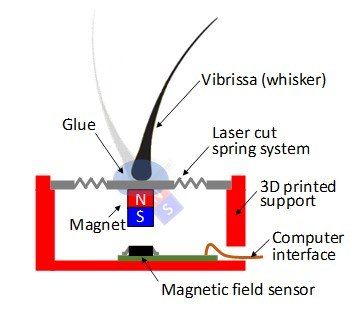
\includegraphics[width=\textwidth]{figures/kim-velez-whisker}
        \caption{Magnetically transduced whisker sensing mechanism schematic by \textcite{8968518}.}
        \label{fig:kim-whisker}
    \end{subfigure}\hfill
    \begin{subfigure}{0.48\textwidth}
        \centering
        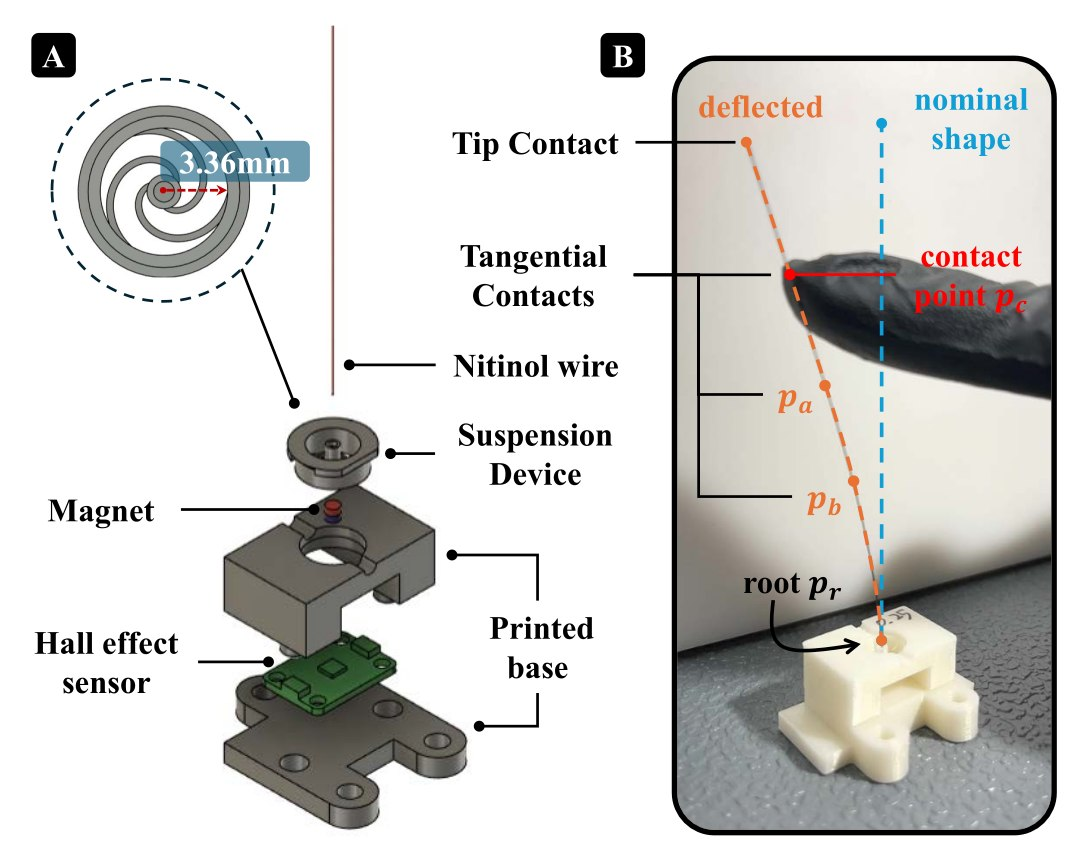
\includegraphics[width=\textwidth]{figures/dang-whisker}
        \caption{Structure of whisker-inspired tactile sensor by \textcite{dang2025whisker}.}
        \label{fig:dang-whisker}
    \end{subfigure}
    \caption{Side-by-side comparison of whisker sensor designs.}
\end{figure}

\subsection{Piezoresistive Whisker Sensors}
Piezoresistive whisker sensors are the most common type, notably applied in marine robotics to detect water flow and pressure variations.

\textcite{GUO2024114875} developed a Piezoelectric Wavy Whisker Sensor (PWWS) inspired by seal whiskers.
The sensor consists of a flexible, waterproof Polydimethylsiloxane (PDMS) body and a thin sensing layer made of Polyvinylidene Difluoride (PVDF).
PDMS, a rubber-like material, protects the sensor from water, while PVDF is a polymer generating a small electrical voltage when bent or pressed.
When water flows around an object, vortices form, pushing against the whisker, bending the PVDF layer, and producing a voltage as depicted in Figure~\ref{fig:piezoelectric-whisker}.
The generated voltage correlates with water flow parameters, enabling tracking of underwater disturbances.

\begin{figure}[htb]
    \centering
    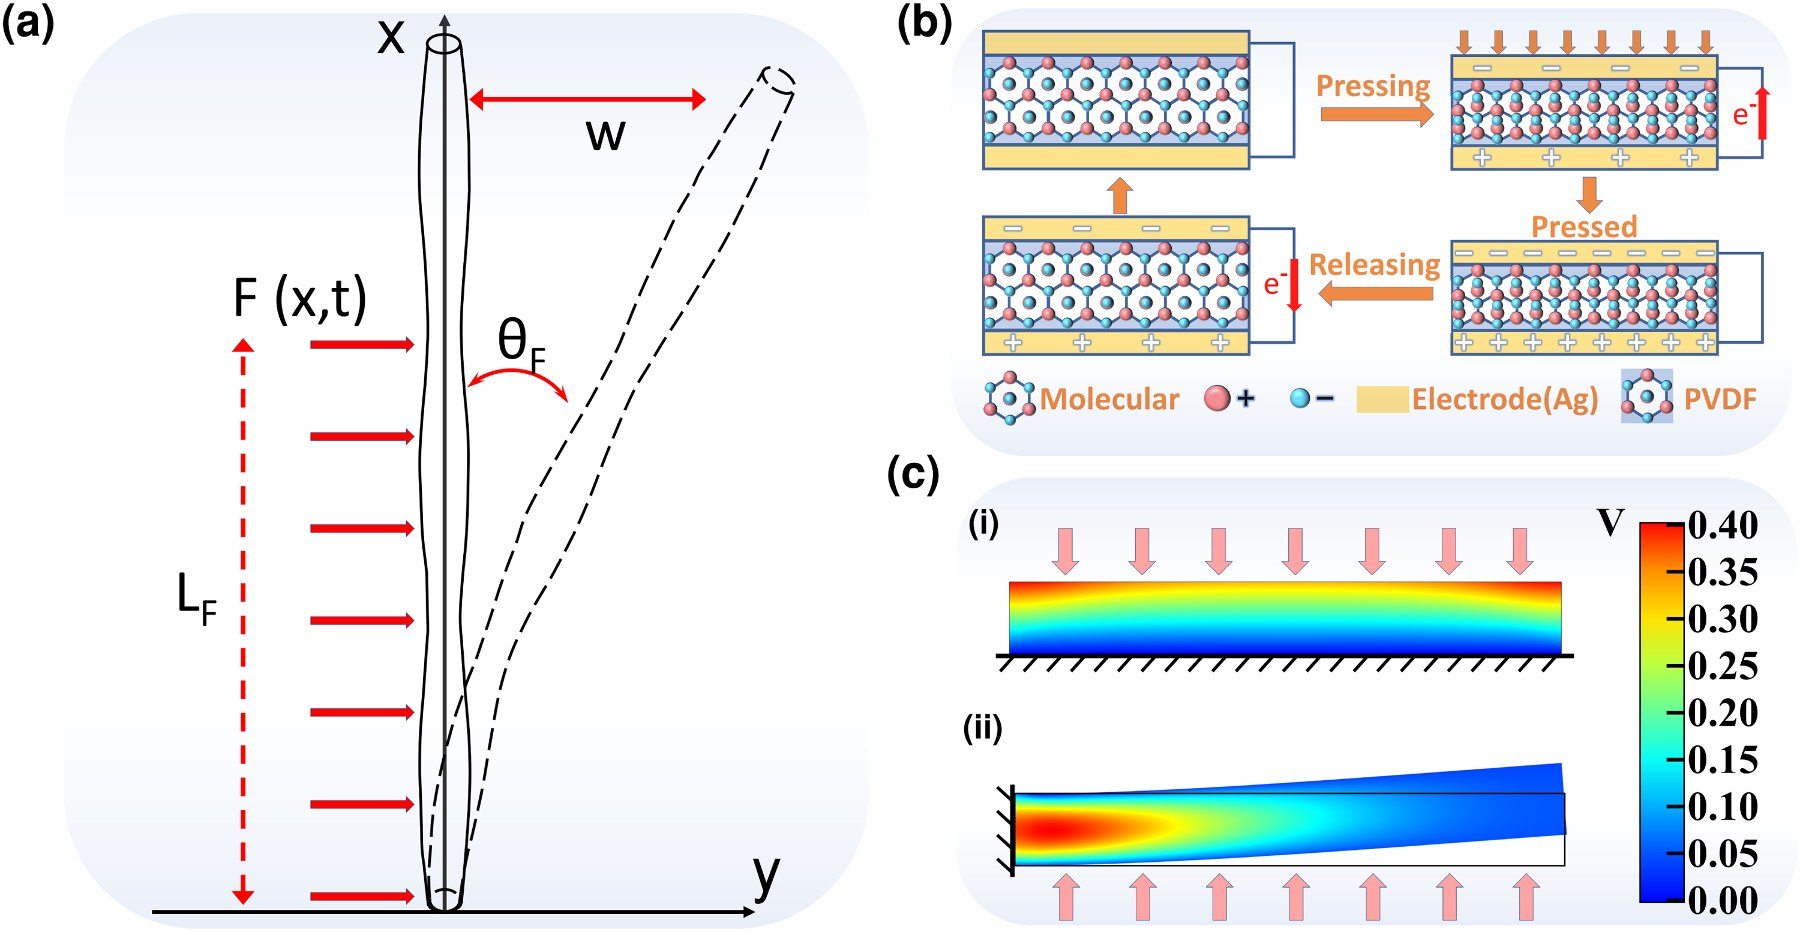
\includegraphics[width=\textwidth]{figures/piezoelectric-whisker}
    \caption{Operating principles of the PWWS by \textcite{GUO2024114875}. (a) Schematic of whisker deflection under force. (b) Cycle of electrical signals generated by the piezoelectric sensing unit. (c) Simulation of piezoelectric voltage within PVDF material under various constraints when subjected to external forces.}
    \label{fig:piezoelectric-whisker}
\end{figure}

\subsection{MEMS Whisker Sensors}
\textcite{9114501} developed a MEMS-based biomimetic whisker sensor replicating the tactile sensing mechanism of rats.
The sensor is integrated onto a small silicon chip (\SI{6.8}{\milli\meter\squared}) containing four identical sensing units.
Each unit mimics the follicle arrangement of a rat's whisker, featuring a flexible whisker shaft attached to a central hub and four beams.
Piezoresistors implanted on these beams form a Wheatstone bridge.
Whisker bending from contact changes the resistance, producing an electrical signal.
The sensor fabrication uses standard MEMS processes, and the resulting structure is shown in Figure~\ref{fig:mems-whisker}.
Production begins with an Silicon-on-Insulator (SOI) wafer, followed by ion implantation, insulating and metal layer deposition, and beam etching.
Experiments indicate the sensor reliably measures contact distances (\qtyrange{30}{40}{\milli\metre}), recognizes object shapes (round, flat, beveled), and differentiates textures.
Thus, this whisker sensor has significant potential for integration into robotic systems requiring tactile sensing.

\begin{figure}[htb]
    \centering
    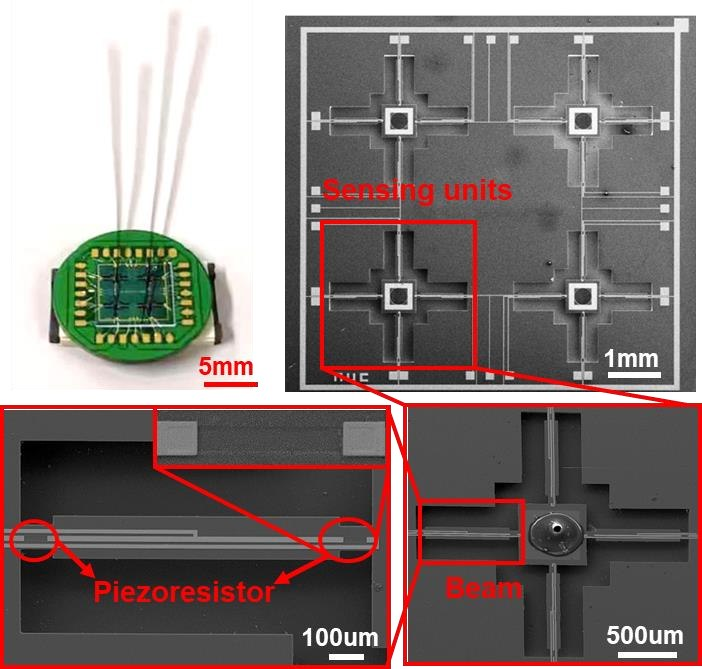
\includegraphics[height=0.4\textheight]{figures/mems-whisker}
    \caption{SEM image of the MEMS-based biomimetic whisker sensor by \textcite{9114501}.}
    \label{fig:mems-whisker}
\end{figure}

\subsection{Contour Reconstruction}
Whisker sensors are particularly suited to contour reconstruction due to their precise contact localization capabilities.
However, two main issues affect their application:

\begin{enumerate}
    \item Detachment or slippage of the whisker due to varying surface textures.
    \item Inability to distinguish between tangential and normal contact.
\end{enumerate}

Detachment or slippage issues can be mitigated using active control policies that actively reestablish whisker contact upon detachment.
Distinguishing tangential from normal contacts can be addressed by additionally considering torque measurements alongside bending moments, as described by~\cite{doi:10.1089/soro.2016.0028}, but this approach is considerably more complex for practical implementation.


\section{Active Tactile Exploration}
Active tactile exploration is a technique in robotics for gathering environmental information through touch.
Typical applications include contact localization~\cite{doi:10.1089/soro.2016.0028}, contour reconstruction~\cite{lin2022whiskerinspiredtactilesensingcontact}, object recognition~\cite{Xiao_2022}, and manipulation~\cite{Brouwer2024TactileInformedAP}.
Whisker sensors, discussed in the previous section, offer a promising solution for these tasks.

\subsection{Contour Reconstruction}
Research on whisker-based active tactile exploration includes the work by \textcite{dang2025whisker}, which introduces both a whisker sensor and an accompanying control system for active tactile exploration.
In their work, the whisker is actuated by a Franka Emika Panda robotic arm for object contour reconstruction.
The control approach involves the following steps:
\begin{enumerate}
    \item Hall sensor data from the whisker sensors is processed to determine the whisker tip position, with noise reduced using Kalman filtering.
    \item A spline is fitted through the last $N$ whisker tip position measurements to calculate the curvature of the whisker.
    \item The desired whisker rotation aligns with the surface normal at the next predicted contact point from the spline.
    \item A PID controller maintains a constant whisker deflection profile.
    The controller adjusts the whisker's normal velocity based on the deflection error, compressing or relaxing the whisker as needed by moving along the surface normal.
    \item The tangential velocity component is adjusted so that the total velocity remains constant.
\end{enumerate}

This approach achieves excellent results, reconstructing smooth surfaces with submillimeter accuracy.
Small sharp angles can also be navigated, provided the whisker does not detach.

However, whisker detachment remains a significant challenge, as sudden, unpredictable slips inevitably occur, necessitating a retrieval mechanism.
Another limitation of the approach of \citeauthor{dang2025whisker} is the inherent instability in contour tracking direction--small disturbances may cause unintended reversal in exploration direction.
Nevertheless, this control policy forms a solid foundation for developing more robust solutions, including retrieval strategies.

\subsection{Environment Manipulation}
When the sensory array is reliable enough, complex manipulation tasks can be performed.
\textcite{Brouwer2024TactileInformedAP} have developed tactile-informed action primitives designed to help robots reach targets in densely cluttered environments without getting stuck.
Their approach introduces two simple motion patterns: the \enquote{burrow} primitive adds a gentle, snaking side-to-side motion to clear a path, while the \enquote{excavate} primitive makes a spiraling, scooping motion that pushes obstacles aside.
Both primitives are depicted in Figure~\ref{fig:environment-manipulation}.
By integrating these primitives into a closed-loop control strategy informed by soft tactile sensors on the robot's finger-like end-effector, the system can sense contact forces and adjust its motion in real time.
Both simulation and hardware experiments show that this strategy dramatically improves performance--reducing both the distance to the goal and the time to complete the reach--and significantly increases the success rate compared to traditional straight-line motion.

\begin{figure}[htb]
    \centering
    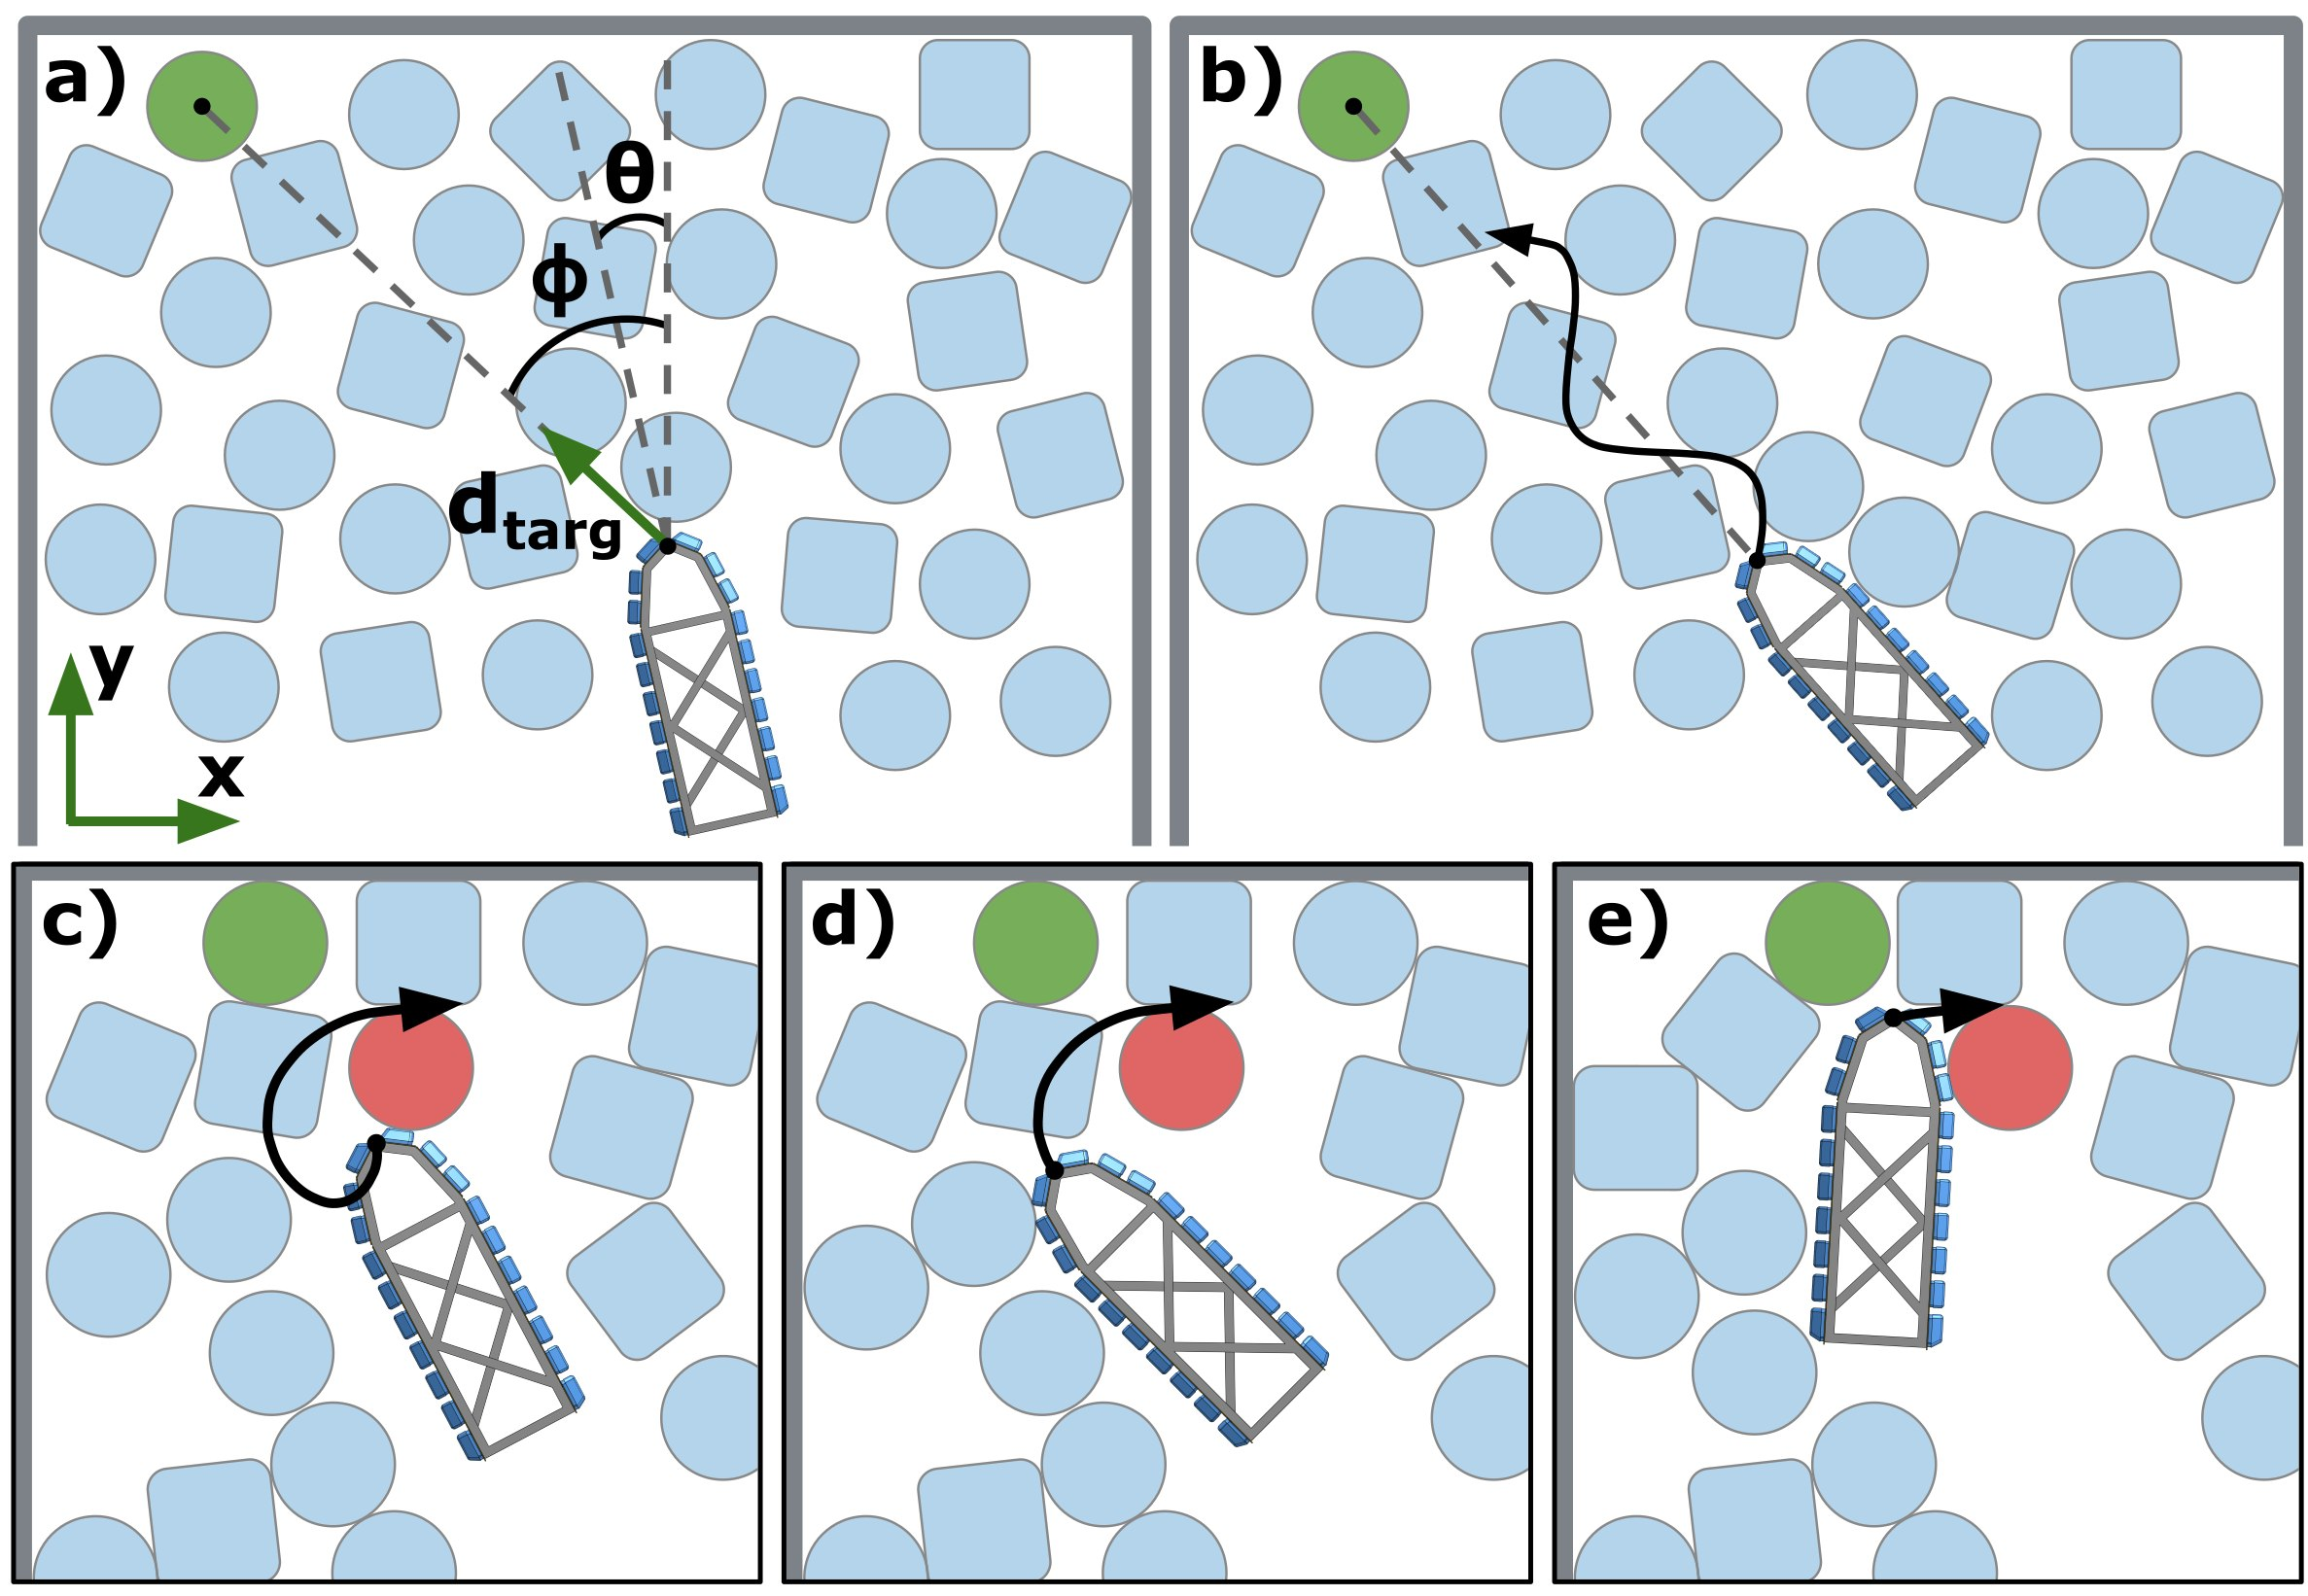
\includegraphics[width=\textwidth]{figures/environment-manipulation}
    \caption{Schematic visualizations of a) straight line control, b) burrowing action primitive and c--e) a sequence showing the progression of a clockwise excavate action primitive, by \textcite{Brouwer2024TactileInformedAP}.}
    \label{fig:environment-manipulation}
\end{figure}